\chapter{Einleitung}

\section{Der Projektkontext}

Die Arbeit am Projekt Muminav begann im Mai 2002 im Rahmen einer
Lehrveranstaltung an der TU-Berlin\footnote{{http://www.tu-berlin.de}}. Es
handelt sich dabei um die Realisierung eines Teils des ebenfalls an der
TU-Berlin laufenden Projektes  \glqq Multimediale Mathematikausbildung f�r
Ingenieure\grqq\ \footnote{kurz: \textsc{Mumie}} \cite{Mumie}.

\subsection{Dezentrale Systementwicklung am Beispiel GNU/Linux}

Die Lehrveranstaltung \glqq Dezentrale Systementwicklung am Beispiel
GNU/Linux \grqq\ \cite{DESE}, die am Institut f�r
Elektrotechnik und Informatik\footnote{{http://cs.tu-berlin.de}} angeboten wird,
soll den Teilnehmern einen Einblick in die dezentrale Entwicklung von
Softwaresystemen verschaffen. Der Schwerpunkt liegt auf der Betrachtung von Open
Source Software.

Der theoretische Teil umfasst Themen wie die Geschichte und Philosophie von Open
Source Software (im Speziellen GNU/Linux), Parallelen zwischen
Wissenschafts- und Entwicklungstheorien zum Ent- und Bestehen von freien
Softwaresystemen, die Organisation und Eigenheiten entsprechender Projekte und
die damit verbundenen Anforderungen an die Entwickler, Hilfsmittel, die die
dezentrale Entwicklung unterst�tzen und einige andere mehr.

F�r den praktischen Teil bearbeiten die Teilnehmer ein Projekt, um selbst
Erfahrungen auf dem Gebiet der dezentralen Systementwicklung zu sammeln. Es
werden vom Veranstalter Projektphasen vorgegeben, zu denen Vortr�ge und
Ausarbeitungen den Stand der Entwicklung wiederspiegeln sollen. Die Entwicklung
soll durch die Nutzung von in diesem Bereich bekannten Tools (z.B.
Mailinglisten, CVS, Homepage etc.) unterst�tzt werden und es wird die 
Wiederbenutzung schon bestehender Software angeregt. Ziel ist es, zum Abschluss
der Veranstaltung einen Prototypen des Systems vorzustellen.

Die Inhalte der Projekte stehen den Teilnehmern v�llig frei. Sie suchen sich
selbst ein Thema oder arbeiten mit einem externen Auftraggeber
zusammen. Daf�r werden auch einige Kontakte vom Veranstalter hergestellt
und angeboten.

\subsection{Das Projekt Mumie}

\glqq Multimediale Mathematikausbildung f�r Ingenieure\grqq\ ist ein vom
Bundesministerium f�r Bildung und Forschung gef�rdertes Projekt, dass an der
TU-Berlin in Kooperation mit 3 weiteren deutschen Universit�ten entwickelt wird.

Das Ziel liegt in der Entwicklung einer WWW-basierten, modularen Umgebung, die
einerseits dem Lernendem den Zugang zur Mathematik und andererseits dem Dozenten
die Vermittlung von Wissen durch den Einsatz moderner, multimedialer
Techniken erleichtern soll. Das System soll aus mehreren Modulen bestehen:

\begin{itemize}
\raggedright
\item Darstellung mathematischer Inhalte mit interaktiver
Multimedia-Unterst�tzung
\item Stoffnachbereitung, Wiederholungsunterst�tzung angeleitete und kommen\-tier\-te
�bungs\-auf\-gaben
\item Selbstkontrolle durch individuelle
Testumgebungen
\item Einf�hrung in mathematische Standardsoftwarepakete
\item individuelles Trainingscenter weiterf�hrender
Inhalte
\item Informationsplattform in der und vile und in die der es auch
noch kein wer, was, wie, wo
\item Kommunikations-- und
Austauschangebote
\end{itemize}

Zus�tzlich werden Schwerpunkte auf eine individualisierbare Oberfl�che und eine
intelligente Benutzerf�hrung gesetzt, um den Benutzern einen einfachen Umgang
mit dem Stoff zu erm�glichen.

\section{Ziele}

Ein Dozent soll die M�glichkeit haben, aus einer Auswahl an
Elementen \footnote{Motivation, Definition, Theorem, Lemma,
Algorithmus, Anwendung}, die in einer Datenbank gespeichert sind,
die Zusammenstellung f�r einen Kurs zu erstellen. Dies soll durch
einfaches Ziehen und Ablegen von Elementsymbolen auf einer
Zeichenfl�che erfolgen. Zusammenh�nge zwischen Elementen werden
dabei durch Verbindungslinien dargestellt, die der Verfasser
positionieren kann. Zus�tzlich kann es zu den Elementen
Subelemente \footnote{Herleitung, Beweis, Motivation, Bemerkung,
Historisches, Visualisierung, Beispiel, Tabelle} geben. Es
entsteht durch die Zusammenstellung eine Repr�sentation der
mathematischen Zusammenh�nge mittels eines gerichteten Graphen.
Der Dozent kann zur Darstellung des Kursverlaufes eine Art \glqq
roten Faden\grqq\ festlegen, der allerdings nicht entlang der
angelegten Verbindungen laufen muss \footnote{Aktueller Stand,
�nderungen m�glich}.

Die Aufgabe f�r das Projekt \textsc{MumiNav} besteht darin, dieses
vorgegebene Netz mit Hilfe eines Java-Applets in einem
Navigationsframe darzustellen und somit den Zugriff auf die
Inhalte zu erm�glichen. Die Darstellung der Elemente erfolgt durch
unterschiedlich farbige, leicht dreidimensional angedeutete
K�sten. Subelemente werden nach vorgeschriebenen Regeln an diesen
K�sten angeordnet und sind standardm��ig nicht mit
Unterscheidungsmerkmalen versehen.

\begin{figure}[htbp]
    \centering%
%   \setcapwidth[c]{12cm}%
    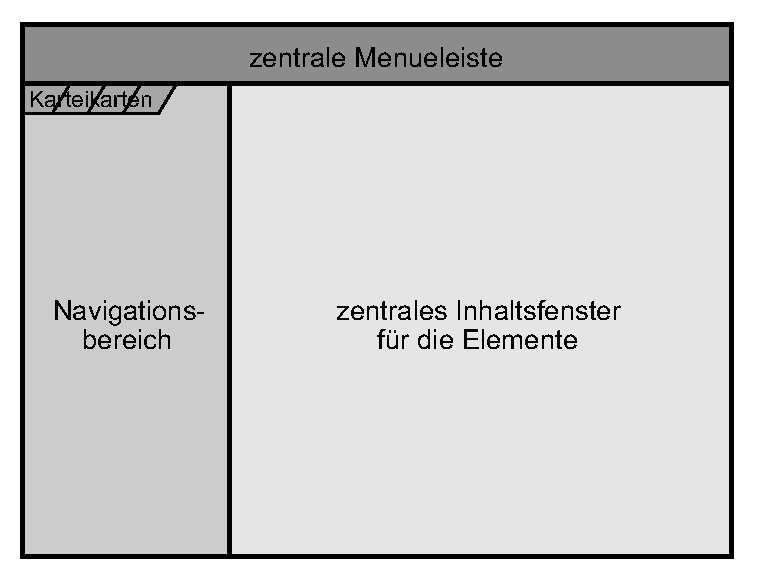
\includegraphics[width=8cm]{figs/haupframe}
    \captionbelow{Layout der Hauptansicht}
    \label{FIG:Hauptansicht}
\end{figure}

Die Abbildung des logischen Netzes geschieht, wie vorher
beschrieben, durch Verbindungslinien zwischen den Elementsymbolen.
Es wird ein \glqq roter Faden\grqq\ entsprechend der linearen
Anordnung der Kursinhalte gelegt.

\begin{figure}[htbp]
    \centering%
%   \setcapwidth[c]{12cm}%
    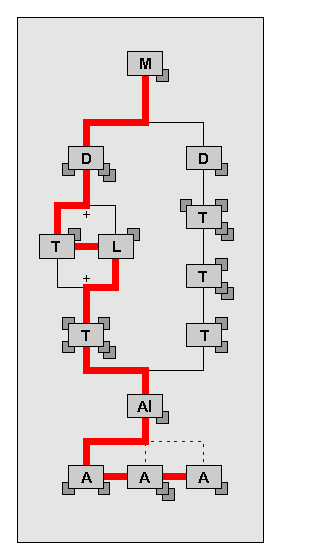
\includegraphics[height=7cm]{figs/navinetz}
    \captionbelow{Kurspfade und roter Faden}
    \label{FIG:roterFaden}
\end{figure}

Die Darstellung soll auf mehrere Maus-Aktionen reagieren. Wird die
Maus �ber ein Element bewegt, soll dieses vergr��ert dargestellt
werden und die Subelemente werden unterscheidbar durch
Beschriftung. Bei Klick mit der linken Maustaste soll der Inhalt
des jeweiligen (Sub-)Elementes im zentralen Inhaltsfenster
dargestellt werden. Dieselbe Aktion auf der mittleren Maustaste
f�hrt zu einem �ffnen des Inhalts in einem externen Fenster und
schlie�lich ist es zuk�nftig vorgesehen, mit der rechten Maustaste
eine Liste von Optionen anzubieten.

\begin{figure}[htbp]
    \centering%
%   \setcapwidth[c]{12cm}%
    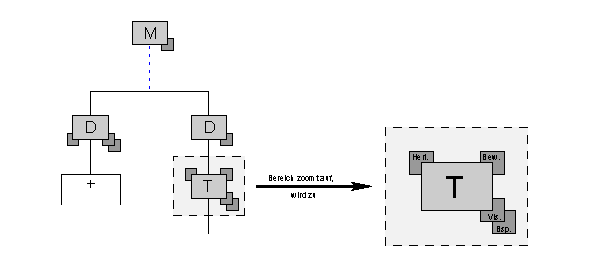
\includegraphics[width=10cm]{figs/zoom_element}
    \captionbelow{Detailansicht bei Zoom}
    \label{FIG:zoomElement}
\end{figure}


